\chapter{Rendering Pipeline}
\begin{figure}[h]
	\centering
	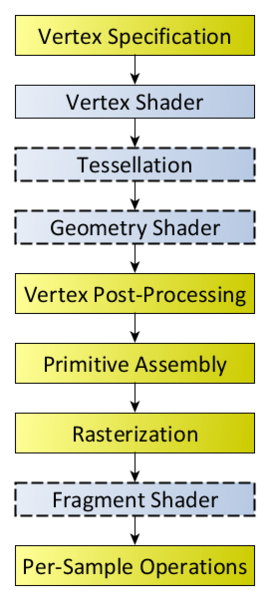
\includegraphics[scale=0.4]{imagens/openglPipeline.png}
	\caption{\small \textit{Rendering pipeline} OpenGL (Fonte: OpenGL, 2016)}
	\label{fig:glpipeline}
\end{figure}

O processo de execução de um programa que exibe resultados em um monitor gráfico requer uma série de etapas, com grande quantidade de cálculos (CLEMENTS, 2014). Assim como na CPU (\textit{Central Processing Unit}, Unidade de Processamento Central), que realiza o processamento geral do computador, a GPU (\textit{Graphics Processing Unit}, Unidade de Processamento Gráfico), também se beneficia de \textit{pipeline}.

Tal processo é definido pela execução paralela de múltiplas etapas, diminuindo a ociosidade do \textit{hardware} e aumentando a taxa de saída de dados (\textit{throuput}) (SHEN e LIPASTI, 2013). Logo que uma primeira instrução é finalizada em uma etapa, uma segunda pode iniciar, desde que não possua outras dependências.

A primeira etapa programável de processamento é o \textit{vertex shader}, sendo também a única obrigatória. Sua função é efetuar cálculos, tendo apenas um vértice como entrada e saída de dados. Para funcionar corretamente, o programador deve especificar a entrada, chamada de \textit{vertex attribute}.

\begin{lstlisting}[caption="AAAAAA"]
	float A;
	
	While{true}{	
		A = 0;
		
		If{A > 60} {
			A = 30;
		}
		A = 20;
	}
}
\end{lstlisting}

%\caption{Exemplo de \textit{vertex shader}.}
\label{alg:vertexattribute}